% Intended LaTeX compiler: xelatex
\documentclass{orgstandard}
\author{ITT-Net-IS}
\date{\today}
\title{Gesetze und Zuständigkeiten in der IT-Sicherheit\\\medskip
\large IT-Sicherheit}
\hypersetup{
 pdfauthor={ITT-Net-IS},
 pdftitle={Gesetze und Zuständigkeiten in der IT-Sicherheit},
 pdfkeywords={},
 pdfsubject={},
 pdfcreator={Emacs 31.0.50 (Org mode 9.7.11)}, 
 pdflang={German}}
\begin{document}

\maketitle
\section{Überblick}
\label{sec:orgadd2fd1}
Dieses Modul behandelt die gesetzlichen Rahmenbedingungen und Zuständigkeiten im Bereich der IT-Sicherheit. Es werden relevante Gesetze, Standards und organisatorische Strukturen vorgestellt, die für die Implementierung und Aufrechterhaltung einer angemessenen qIT-Sicherheit in Unternehmen und Organisationen notwendig sind.
\section{Verantwortliche Stellen und Zuständigkeiten}
\label{sec:org310bfeb}

In einem gut strukturierten Sicherheitsmanagement sind verschiedene Rollen und Verantwortlichkeiten klar definiert:

\begin{center}
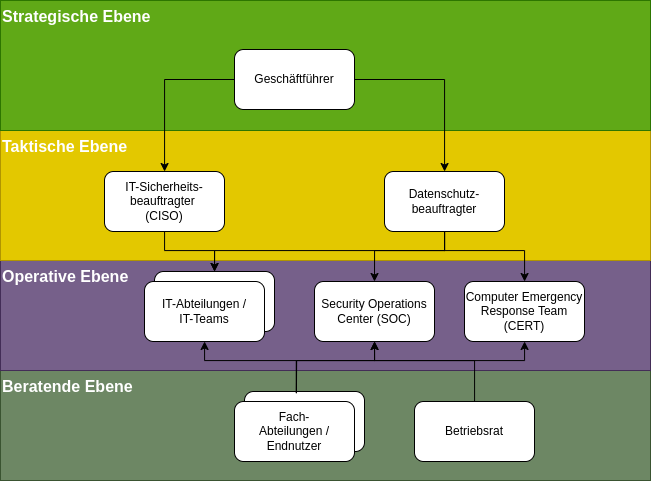
\includegraphics[width=.9\linewidth]{img/Verantwortliche.png}
\end{center}
\subsection{Geschäftsführung}
\label{sec:org182df99}
\begin{itemize}
\item Trägt die Gesamtverantwortung für die IT-Sicherheit
\item Stellt notwendige Ressourcen bereit
\item Verabschiedet die IT-Sicherheitsleitlinie
\item Haftet persönlich für Verstöße gegen gesetzliche Vorschriften
\end{itemize}
\subsection{IT-Sicherheitsbeauftragter (CISO - Chief Information Security Officer)}
\label{sec:org45445f4}
\begin{itemize}
\item Entwickelt und koordiniert das Sicherheitskonzept
\item Berichtet direkt an die Geschäftsführung
\item Überwacht die Umsetzung von Sicherheitsmaßnahmen
\item Berät in Sicherheitsfragen
\item Führt Risikoanalysen durch
\item Erarbeitet Notfallpläne
\end{itemize}
\subsection{Datenschutzbeauftragter}
\label{sec:orgcb1a022}
\begin{itemize}
\item Überwacht die Einhaltung des Datenschutzrechts
\item Berät bei datenschutzrechtlichen Fragen
\item Prüft Verfahren zur Verarbeitung personenbezogener Daten
\item Ist weisungsfrei und berichtet direkt an die Geschäftsleitung
\end{itemize}
\subsection{IT-Abteilung}
\label{sec:org8f8b2ef}
\begin{itemize}
\item Setzt technische Sicherheitsmaßnahmen um
\item Betreibt die Systeme nach Sicherheitsvorgaben
\item Reagiert auf Sicherheitsvorfälle
\item Führt regelmäßige Updates und Backups durch
\end{itemize}
\subsection{Fachabteilungen/Benutzer}
\label{sec:org4cfd7d4}
\begin{itemize}
\item Melden Sicherheitsvorfälle
\item Halten sich an Sicherheitsrichtlinien
\item Tragen durch ihr Verhalten wesentlich zur Gesamtsicherheit bei
\end{itemize}
\subsection{Betriebsrat}
\label{sec:orgc121a27}
\begin{itemize}
\item Vertritt die Interessen der Mitarbeiter bei Sicherheitsrichtlinien
\item Muss bei überwachungsrelevanten Maßnahmen einbezogen werden
\end{itemize}
\subsection{Security Operations Center (SOC)}
\label{sec:orgf107de9}
Ein SOC ist eine zentrale Einheit, die für die kontinuierliche Überwachung und Verbesserung der IT-Sicherheitslage zuständig ist:
\begin{itemize}
\item 24/7-Überwachung der Systeme
\item Erkennung von Sicherheitsvorfällen
\item Analyse und Reaktion auf Vorfälle
\item Forensische Untersuchungen
\item Regelmäßige Sicherheitstests
\end{itemize}

\begin{NOTES}
\begin{itemize}
\item \textbf{24/7-Überwachung:} Permanente Kontrolle von IT-Systemen, um Bedrohungen frühzeitig zu erkennen.
\item \textbf{Forensische Untersuchungen:} Analyse von Sicherheitsvorfällen zur Identifikation von Ursachen und Tätern.
\item \textbf{Sicherheitstests:} Regelmäßige Tests zur Identifikation und Behebung von Sicherheitslücken.
\end{itemize}
\end{NOTES}
\subsection{Computer Emergency Response Team (CERT)}
\label{sec:orgf183a6e}
Ein CERT oder CSIRT (Computer Security Incident Response Team) ist darauf spezialisiert, auf IT-Sicherheitsvorfälle zu reagieren:
\begin{itemize}
\item Sofortmaßnahmen bei Sicherheitsvorfällen
\item Unterstützung bei der Wiederherstellung von Systemen
\item Analyse von Angriffsvektoren
\item Informationsaustausch mit anderen CERTs
\end{itemize}

\begin{NOTES}
\begin{itemize}
\item \textbf{Angriffsvektoren:} Wege und Methoden, über die ein Angriff auf ein IT-System erfolgen kann.
\item \textbf{Informationsaustausch mit anderen CERTs:} Zusammenarbeit mit anderen Sicherheitsorganisationen zur schnelleren Bedrohungserkennung.
\end{itemize}
\end{NOTES}
\section{Gesetze und Standards zur Informationssicherheit}
\label{sec:org8026ccf}

In der digitalen Welt gewinnen Gesetze und Standards zur IT-Sicherheit an Bedeutung. Angesichts wachsender Cyberbedrohungen sind die rechtlichen Anforderungen verschärft worden, da IT-Sicherheit nicht nur eine technische, sondern auch eine unternehmerische und gesellschaftliche Verantwortung ist.

\begin{NOTES}
Unternehmen müssen nationale und internationale Vorschriften einhalten, die oft nur Mindeststandards definieren. Verstöße können hohe Strafen, Haftung für Führungskräfte und Reputationsverluste nach sich ziehen. Neben gesetzlichen Vorgaben spielen internationale Standards eine wichtige Rolle, da sie strukturierte Ansätze zur Informationssicherheit bieten und Vertrauen schaffen. Im Folgenden werden zentrale gesetzliche Regelungen und Standards vorgestellt.
\end{NOTES}
\subsubsection{Datenschutz-Grundverordnung (DSGVO)}
\label{sec:org1915fd9}
\begin{itemize}
\item Europäische Verordnung zum Schutz personenbezogener Daten
\item Verpflichtet zur Implementierung technischer und organisatorischer Maßnahmen
\item Meldepflicht bei Datenschutzverletzungen (72 Stunden)
\item Hohe Bußgelder bei Verstößen (bis zu 4\% des weltweiten Jahresumsatzes)
\end{itemize}
\subsubsection{NIS2-Richtlinie (Netzwerk- und Informationssicherheit)}
\label{sec:org1eb63a4}
\begin{center}
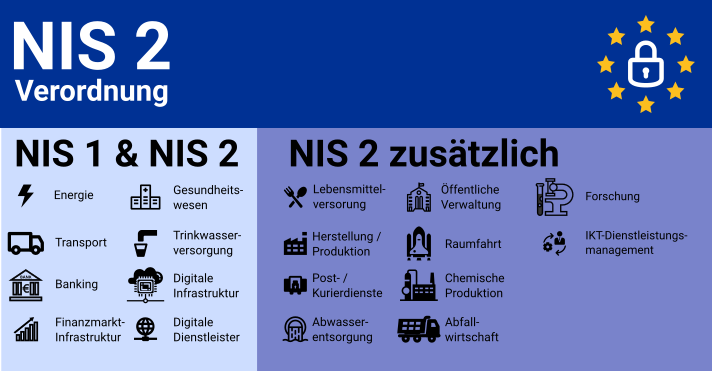
\includegraphics[width=.9\linewidth]{img/NIS2.png}
\end{center}
\begin{itemize}
\item Nachfolger der ersten NIS-Richtlinie aus 2016
\item In Kraft seit Januar 2023 mit Umsetzungsfrist bis Oktober 2024
\item Erweitert den Anwendungsbereich auf weitere Sektoren (Energieversorgung, Verkehr, Finanzdienstleistungen, Gesundheitswesen, öffentliche Verwaltung, Raumfahrt, IKT-Dienstleistungen, u.v.m.)
\item Unterscheidet zwischen "wesentlichen" und "wichtigen" Einrichtungen mit unterschiedlichen Anforderungen
\end{itemize}
\begin{itemize}
\item Stärkere Harmonisierung des Sicherheitsniveaus in der EU
\item Umfassende Meldepflichten für Cybersicherheitsvorfälle
\item Verpflichtung zur Einrichtung von Risikomanagementmaßnahmen
\item Deutlich höhere Bußgelder als bei NIS1 (bis zu 10 Millionen Euro oder 2\% des weltweiten Jahresumsatzes)
\item Stärkere Management-Verantwortung: Die Leitungsorgane müssen Cybersicherheitsschulungen absolvieren und haften persönlich für Verstöße
\end{itemize}
\subsubsection{IT-Sicherheitsgesetz (IT-SiG 2.0)}
\label{sec:org07bd3c2}
\begin{itemize}
\item Regelt insbesondere den Schutz kritischer Infrastrukturen
\item Meldepflicht für Sicherheitsvorfälle
\item Verpflichtung zur Implementierung angemessener Sicherheitsmaßnahmen
\item Erweiterte Befugnisse für das BSI (Bundesamt für Sicherheit in der Informationstechnik)
\item Wird durch die nationale Umsetzung der NIS2-Richtlinie weiterentwickelt
\end{itemize}
\subsubsection{Branchenspezifische Regelungen}
\label{sec:orgb0df9f6}
\begin{itemize}
\item Bankensektor: MaRisk (Mindestanforderungen an das Risikomanagement)
\item Gesundheitswesen: Patientendatenschutzgesetz
\item Telekommunikation: Telekommunikationsgesetz (TKG)
\item Energiesektor: Energiewirtschaftsgesetz (EnWG)
\end{itemize}
\subsection{Internationale Standards und Frameworks}
\label{sec:org6ea22fb}

Im Bereich der IT-Sicherheit haben sich verschiedene internationale Standards und Frameworks etabliert, die Organisationen bei der systematischen Umsetzung von Sicherheitsmaßnahmen unterstützen.

\begin{NOTES}
Diese Standards bieten bewährte Vorgehensweisen, Methoden und Kontrollmechanismen, die über gesetzliche Mindestanforderungen hinausgehen und auf internationalen Best Practices basieren.
\end{NOTES}

Anders als Gesetze sind die meisten Standards \textbf{nicht verpflichtend}, werden aber oft von Kunden, Partnern oder Aufsichtsbehörden erwartet und können einen Wettbewerbsvorteil darstellen.

\begin{NOTES}
Eine Zertifizierung nach anerkannten Standards signalisiert nach außen, dass ein Unternehmen Informationssicherheit ernst nimmt und systematisch angeht.
\end{NOTES}
\subsubsection{ISO/IEC 27001}
\label{sec:org44fe575}
\begin{itemize}
\item Internationaler Standard für Informationssicherheits-Managementsysteme (ISMS)
\item Systematischer Ansatz zur Verwaltung vertraulicher Informationen
\item Basis für Zertifizierungen
\item Umfasst Anforderungen an Planung, Umsetzung, Überwachung und Verbesserung
\end{itemize}
\subsubsection{NIST Cybersecurity Framework}
\label{sec:org83ee369}
\begin{itemize}
\item Von der US-amerikanischen Behörde NIST entwickeltes Rahmenwerk
\item Besteht aus den Kernelementen: Identifizieren, Schützen, Erkennen, Reagieren, Wiederherstellen
\item Flexibel anpassbar an Unternehmensgrößen und -typen
\end{itemize}
\subsubsection{ITIL (Information Technology Infrastructure Library)}
\label{sec:orge1bdf43}
\begin{itemize}
\item Framework für IT-Service-Management
\item Enthält Best Practices für IT-Sicherheit im Kontext des Servicemanagements
\item Umfasst Prozesse wie Incident Management und Problem Management
\end{itemize}
\section{Weiterführende Ressourcen}
\label{sec:org3419a31}
\begin{itemize}
\item \href{https://www.bsi-fuer-buerger.de}{BSI für Bürger}
\item \href{https://www.bsi.bund.de/DE/Themen/Unternehmen-und-Organisationen/Standards-und-Zertifizierung/IT-Grundschutz/IT-Grundschutz-Kompendium/it-grundschutz-kompendium\_node.html}{BSI-Grundschutz-Kompendium}
\item \href{https://www.allianz-fuer-cybersicherheit.de}{Allianz für Cybersicherheit}
\item \href{https://dsgvo-gesetz.de}{DSGVO-Volltext}
\item \href{https://eur-lex.europa.eu/legal-content/DE/TXT/HTML/?uri=CELEX:32022L2555}{NIS2-Richtlinie}
\item \href{https://www.bsi.bund.de/DE/Themen/Regulierte-Wirtschaft/NIS-2-regulierte-Unternehmen/nis-2-regulierte-unternehmen\_node.html}{BSI zu NIS2}
\end{itemize}
\end{document}
